\documentclass[a4paper,12pt]{article}

% Pacchetti necessari
\usepackage{lmodern}  % Font moderno
\usepackage{geometry} 
\usepackage{graphicx}
\usepackage{amsmath}
% Gestione margini
\geometry{a4paper, top=3cm, bottom=3cm, left=3cm, right=3cm}

\begin{document}

% Centratura del contenuto sulla pagina
\begin{titlepage}
    \centering
    \vspace*{1cm} % Spazio dall'alto
    
    {\Large \textbf{Paola Loi (33088A)} \par} % Nome autore
    {\Large \textbf{Loris Palmarin (32349A)} \par}
    \vfill % Spazio flessibile
    
    {\Huge \textbf{Algorithms For Massive Datasets} \par} % Titolo
    \vspace{0.5cm}
    {\LARGE Market Basket Analysis \par}
    \vspace{0.5cm}
    {\LARGE Amazon Book Reviews \par}
    
    \vfill % Spazio flessibile
    
    {\Large March 2025 \par} % Data
    
\end{titlepage}

\newpage
\thispagestyle{empty}
\vspace*{\fill}
\begin{center}  
    I/We declare that this material, which I/We now submit for assessment, is entirely my/our own work and has not been taken from the work of others, save and to the extent that such work has been cited and acknowledged within the text of my/our work, and including any code produced using generative AI systems. I/We understand that plagiarism, collusion, and copying are grave and serious offences in the university and accept the penalties that would be imposed should I engage in plagiarism, collusion or copying. This assignment, or any part of it, has not been previously submitted by me/us or any other person for assessment on this or any other course of study.}
\end{center}
\vspace*{\fill}

\newpage
\tableofcontents
\newpage

\newpage % Inizia una nuova pagina

\section{Introduction} % Titolo della sezione senza numerazione

This project has been developed for the \textit{Algorithms for Massive Datasets} course, taught by Professor Malchiodi during the 2024/25 academic year. The objective is to implement a market-basket analysis using the Amazon Books Reviews dataset. The goal is to extract insights into book co-purchasing patterns by identifying frequent itemsets and generating association rules.

To achieve this, we deploy two well-established algorithms for frequent itemset mining:  
\begin{itemize}
    \item \textit{A-Priori}, a two-pass approach designed to efficiently find frequent itemsets while reducing memory usage.
    \item \textit{SON (Savasere, Omiecinski, and Navathe)}, a MapReduce-based algorithm designed for distributed environments, which finds frequent itemsets in chunks of data before validating them globally.
\end{itemize}

The dataset consists of book reviews, where each user represents a basket, and the books they reviewed form the items. The dataset requires preprocessing to remove inconsistencies and ensure proper structuring for association rule mining. The analysis will focus on book pairs that frequently appear together, measuring their support, confidence, and lift to determine meaningful associations.

The implementation is carried out using Apache Spark to handle large-scale data efficiently, leveraging distributed computing for scalability. The two algorithms will be compared in terms of efficiency and scalability, evaluating their performance as the dataset size increases.

In the subsequent sections, we will discuss the preprocessing steps, algorithm implementation details, experimental results, and a critical analysis of the findings.


\newpage
\section{Data}

\subsection{Data Upload}

The dataset used in this project is automatically downloaded at runtime via the Kaggle API. Two files are retrieved:

\begin{itemize}
    \item \texttt{books\_data.csv}: contains metadata about the books, including title, author, edition, publication year, cover image, and more.
    \item \texttt{books\_ratings.csv}: contains user reviews, including \texttt{user\_id}, \texttt{book\_id}, numerical ratings, and review texts.
\end{itemize}

The dataset is based on Amazon book reviews. Once loaded, the tables appear as follows:

\begin{figure}[h]
    \centering
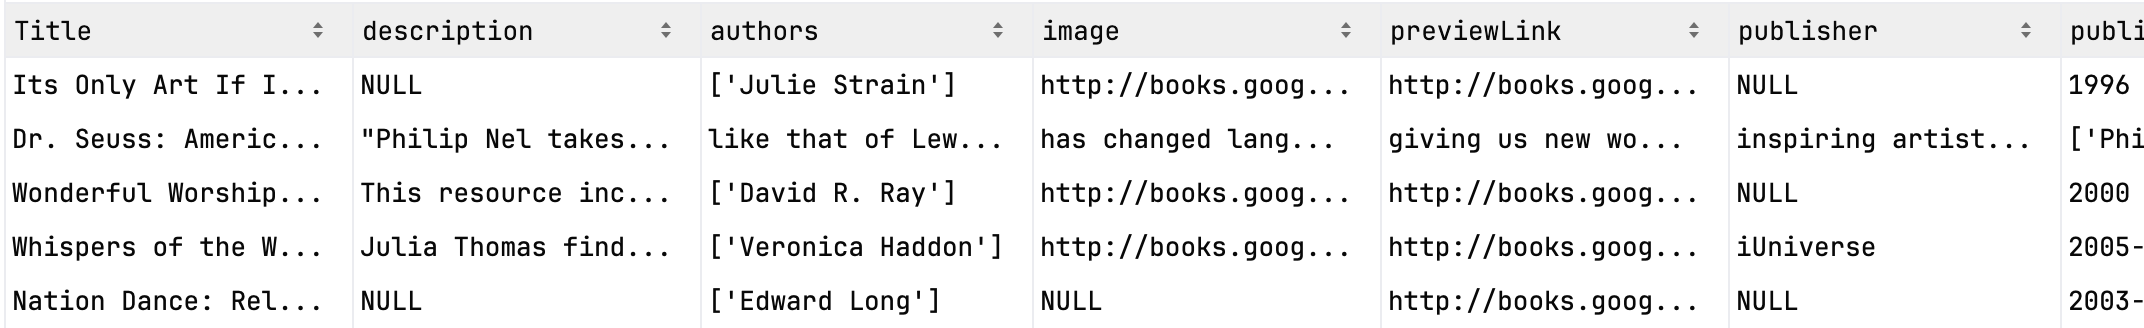
\includegraphics[width=15cm]{images/book_data.png}
    \caption{Preview of books\_data.csv}
\end{figure}
\begin{figure}[h]
    \centering
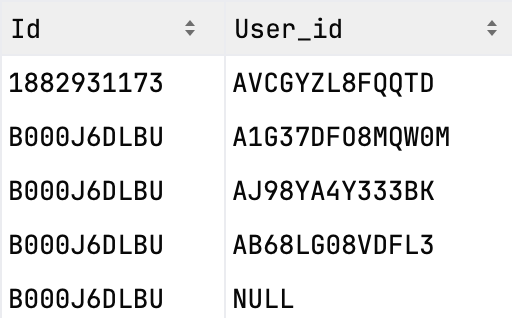
\includegraphics[width=5cm]{images/book_ratings.png}
    \caption{Preview of books\_ratings.csv}
\end{figure}

\subsection{Data Preprocessing}

The tables are loaded into Spark as DataFrames via the SQLContext interface. 
A SQL query is used to select only the relevant columns for market basket analysis—namely, \texttt{user\_id} and \texttt{book\_id} from the \texttt{books\_ratings} table.

\begin{figure}[h]
    \centering
    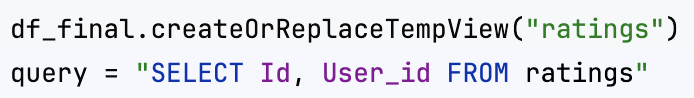
\includegraphics[width=10cm]{images/query.png}
    \caption{Column selection query}
\end{figure}

The full dataset contains approximately 3 million reviews. To reduce computational load during development, a variable \texttt{sampling} is introduced: when set to \texttt{True}, it enables working with just 1\% of the dataset for testing purposes.

The pre-processing phase also includes standard data cleaning steps:

\begin{itemize}
    \item Removal of duplicate entries
    \item Elimination of null values
    \item Merging of books with the same title but different IDs
\end{itemize}

After preprocessing, the dataset is reduced to approximately 2 million cleaned and usable reviews.

\newpage
\section{Algorithms Implementation}

For the purposes of this project, I implemented two different algorithms to find frequent itemsets: A-Priori and SON.

\subsection{A-Priori Algorithm}
\subsubsection{In theory}

The A-Priori algorithm is a classical method for discovering frequent itemsets in transactional datasets, particularly suitable when the number of possible item combinations is too large to be held entirely in memory. A-Priori proceeds in two sequential passes over the dataset to limit the number of candidate itemsets that need to be counted.

\paragraph{First Pass.}  
In the first pass, the algorithm focuses on identifying frequent singleton items:
\begin{enumerate}
    \item Each item is optionally mapped to a unique integer ID.
    \item An array of counts is initialized, where each position corresponds to a specific item.
    \item As the dataset is scanned, each item's count is incremented whenever it appears in a basket.
\end{enumerate}
At the end of this phase, only items whose counts exceed the support threshold $s$ are retained as \textit{frequent singleton items}.

\paragraph{Between Passes.}  
A new mapping is created that assigns new consecutive integer IDs (from 1 to $m$) exclusively to the frequent items identified during the first pass. This enables the algorithm to reduce the memory footprint by focusing only on the relevant items.

\paragraph{Second Pass.}  
During the second pass, the algorithm counts the occurrences of item pairs, but only those composed of items that are already known to be frequent:
\begin{enumerate}
    \item For each basket, the frequent-items mapping is used to filter out infrequent items.
    \item A nested loop is used to generate all possible unordered pairs of the remaining items in the basket.
    \item Each pair is counted using a suitable data structure (e.g., triangular matrix or hash-based table).
\end{enumerate}
At the end of this second pass, the support counts of all candidate pairs are evaluated, and only those that satisfy the minimum support threshold $s$ are retained as frequent pairs.

\subsubsection{Implementation}

The A-Priori algorithm has been implemented using the \texttt{PySpark} package in order to leverage distributed computing and parallelization. Given the size of the dataset and the computational complexity of frequent itemset mining, the use of Spark allows for an efficient and scalable approach to processing large volumes of data.

To begin, the data has been organized into an RDD named \texttt{book\_baskets}. Using PySpark’s \texttt{map} and \texttt{groupByKey} functions, the ratings have been transformed so that each entry in the RDD corresponds to a single user and a list of all book identifiers they have rated. This list of books for each user represents a \textit{basket} in the context of market basket analysis.

Once the baskets were created, we computed the total number of baskets, which resulted in \texttt{1,008,423} entries. This constitutes the dataset over which the A-Priori algorithm is applied in the subsequent steps.

\paragraph{First Pass: Frequent Singletons}

The first pass of the A-Priori algorithm aims to identify the frequent singleton itemsets, i.e., individual books that appear frequently across user baskets. To accomplish this, we define an RDD named \texttt{single\_counts}, which is derived from \texttt{book\_baskets} using PySpark’s \texttt{flatMap} and \texttt{reduceByKey} transformations.

Initially, each book within every basket is isolated and mapped to a key-value pair \texttt{(book\_id, 1)}. Then, using the \texttt{reduceByKey} function, the algorithm aggregates these pairs by summing up the occurrences of each book across all baskets, effectively counting how many times each book appears in the dataset.

To determine which books are frequent, we introduce a support threshold. This threshold is computed as the product between a predefined percentage of the total baskets and the total number of baskets itself. In this implementation, we chose a threshold of 0.001, i.e., books that appear in at least 0.1\% of the baskets are considered frequent.

After applying this filtering step, 81 frequent singleton books were identified in the complete dataset. These were then sorted in descending order of frequency. Notably, the most frequent book appeared in more than 3,000 baskets.

\paragraph{Second Pass: Frequent Pairs}

The second pass replicates the structure of the first pass but focuses on identifying frequent \textit{pairs} of items instead of singletons. To ensure computational efficiency, only the frequent singleton items obtained from the first pass are considered when forming pairs. This step is crucial since, according to the A-Priori principle, a pair can only be frequent if both of its items are themselves frequent.

Using \texttt{flatMap}, all possible unordered pairs of frequent singleton books within each basket are generated. These pairs are mapped to key-value pairs of the form \texttt{((book\_i, book\_j), 1)} and then aggregated via \texttt{reduceByKey} to count their occurrences across all baskets.

The resulting counts are filtered using the same support threshold adopted for the singletons (0.001 of the total number of baskets), yielding 84 frequent pairs. As in the first pass, the final list is sorted in descending order by frequency. The most frequent pair appears 3,574 times in the dataset.

\paragraph{Third Pass: Frequent Triplets}

In the third pass, the algorithm extends the previous procedure to compute frequent \textit{triplets} of books. Again, combinations are generated exclusively from the frequent singleton items, applying the \texttt{flatMap} and \texttt{reduceByKey} operations analogously to the previous passes.

The same support threshold is applied to identify frequent triplets. After filtering and sorting, a total of 111 frequent triplets were found. The most common triplet appears 3,561 times in the dataset.
\paragraph{}
The results will be used in the last section when we will compute the association rules to identify patterns and purchase behavior. 


\newpage

\subsection{SON Algorithm}

\subsubsection{In theory}
The SON (Savasere, Omiecinski, Navathe) algorithm is a two-pass, distributed approach to finding frequent itemsets in large-scale datasets. It is designed to work efficiently in parallel computing environments and eliminates both false positives and false negatives by structuring the process into two key MapReduce phases.
\paragraph{}
In the first pass, the input dataset is divided into smaller chunks (e.g., via partitions in a distributed file system). For each chunk, a local version of the frequent itemset mining algorithm is executed using a lowered support threshold ps, where p is the fraction of data represented by the chunk and s is the global support threshold. This phase yields locally frequent itemsets which are considered as candidate itemsets.
\paragraph{}
In the second pass, the global support for these candidate itemsets is computed by scanning the entire dataset. Only the itemsets that meet or exceed the original support threshold s across the full dataset are retained as globally frequent itemsets.
\paragraph{}
This two-pass structure ensures that:
\begin{itemize}
    \item All globally frequent itemsets are discovered (no false negatives).
    \item The process can be parallelized, improving computational efficiency on large datasets.
\end{itemize}


\subsubsection{Implementation (Map-Reduce version)}


The SON algorithm was implemented using the \texttt{PySpark} framework in order to exploit distributed computing and achieve efficient processing of large-scale datasets. The overall procedure follows the canonical structure of the algorithm and is divided into two MapReduce phases, each executed across multiple data partitions.

\paragraph{First Phase – Local Frequent Itemsets}

In the first phase, the dataset containing user baskets was divided into 10 partitions. Each partition was treated as an independent sample of the global dataset. A local support threshold was computed as:
\[
s_{\text{local}} = s \cdot p
\]
where $s$ is the global support threshold, and $p$ is the fraction of the dataset in a single partition.

Within each partition, the algorithm:
\begin{itemize}
    \item Counted the occurrences of singleton and pair itemsets.
    \item Selected locally frequent itemsets, i.e., those whose count exceeded $s_{\text{local}}$.
    \item Returned these itemsets as candidates for the second phase.
\end{itemize}

At the end of the first MapReduce phase, the set of global candidate itemsets was obtained by computing the union of all locally frequent itemsets. This guarantees that all globally frequent itemsets are preserved, with no false negatives.

\paragraph{Second Phase – Global Support Counting}

In the second phase, the algorithm measured the actual support of each candidate itemset across the full dataset. Each partition contributed to the total count of each candidate.

The second phase involved:
\begin{itemize}
    \item Scanning each basket to check whether it contains each candidate itemset.
    \item Aggregating partial counts across partitions.
    \item Filtering itemsets whose total count exceeded or equaled the global support threshold $s$.
\end{itemize}

The output of this phase is the final set of globally frequent itemsets.

\begin{figure}[h]
    \centering
    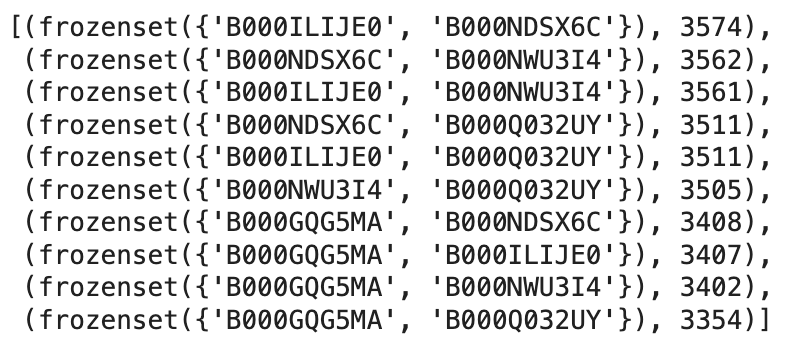
\includegraphics[width=9cm]{images/SON.png}
    \caption{Frequent pairs}
\end{figure}

\newpage
\section{Association Rules}

\subsection*{Association Rules}

Association rules are a fundamental tool in market-basket analysis, used to uncover relationships and dependencies between items in large transactional datasets. Their primary purpose is to identify patterns in purchasing behavior, enabling insights into how the presence of certain items in a basket affects the likelihood of other items being present.

In this project, the association rules are derived from the output of the Apriori algorithm, applied frequent item pairs. By analyzing these frequent itemsets, we can generate rules of the form $A \Rightarrow B$, where $A$ and $B$ are itemsets, and evaluate their strength based on the following key metrics:

\begin{itemize}
    \item \textbf{Support:} Measures how frequently an itemset appears in the dataset.
    \[
    \text{Support}(A) = \frac{\text{Count}(A)}{\text{Total Transactions}}
    \]
    
    \item \textbf{Confidence:} Represents the conditional probability that itemset $B$ appears in a transaction given that $A$ is also present.
    \[
    \text{Confidence}(A \Rightarrow B) = \frac{\text{Support}(A \cup B)}{\text{Support}(A)}
    \]
    
    \item \textbf{Lift:} Indicates how much more likely itemset $B$ is to appear with $A$ compared to if $B$ were independent of $A$.
    \[
    \text{Lift}(A \Rightarrow B) = \frac{\text{Confidence}(A \Rightarrow B)}{\text{Support}(B)}
    \]
\end{itemize}

These metrics help identify the most meaningful and non-trivial associations in the data. Association rules with high confidence and lift are especially useful for practical applications such as recommendation systems and targeted marketing strategies.

\subsection{From pairs}

After computing the metrics described above, this is the final output (only first 5 rules selected:
\begin{figure}[h]
    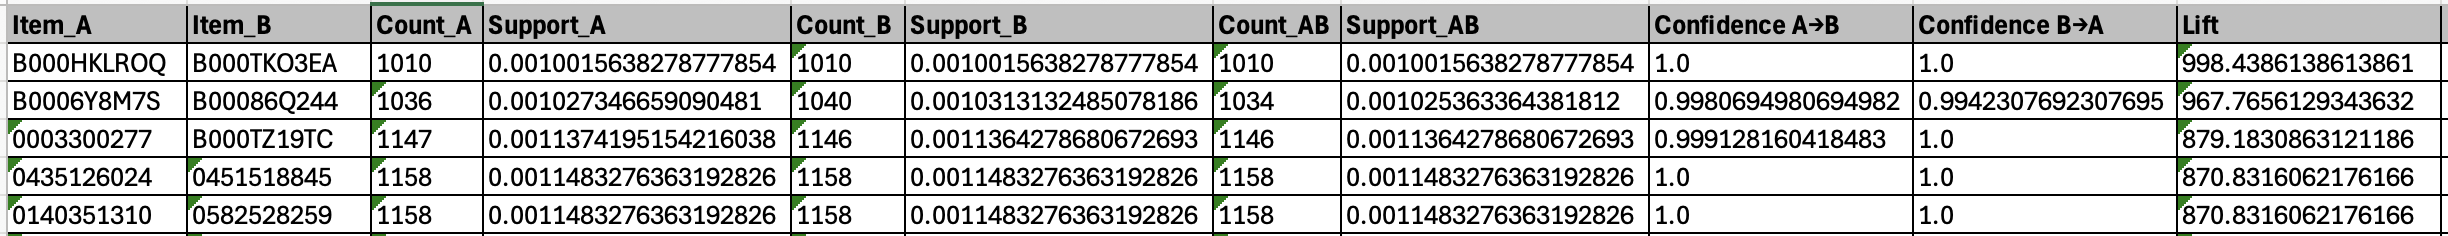
\includegraphics[width=18cm]{images/assoc_rules.png}
    \caption{Column selection query}
\end{figure}

We analyze the top three association rules derived from the most frequent item pairs identified through the \textit{Apriori} algorithm. These rules demonstrate very strong dependencies between items, as indicated by their high confidence and lift values.

\subsubsection*{Rule 1: \texttt{B000HKLROQ} $\Rightarrow$ \texttt{B000TKO3EA}}

\begin{itemize}
    \item \textbf{Support}: 0.0010015
    \item \textbf{Confidence (A $\rightarrow$ B)}: 1.0
    \item \textbf{Confidence (B $\rightarrow$ A)}: 1.0
    \item \textbf{Lift}: 998.44
\end{itemize}

This rule is perfectly symmetric and deterministic — whenever \texttt{B000HKLROQ} appears in a transaction, so does \texttt{B000TKO3EA}, and vice versa. The lift of nearly 1000 confirms an extremely strong association, likely indicating complementary or co-bought items.

\subsubsection*{Rule 2: \texttt{B0006Y8M7S} $\Rightarrow$ \texttt{B00086Q244}}

\begin{itemize}
    \item \textbf{Support}: 0.001025
    \item \textbf{Confidence (A $\rightarrow$ B)}: 0.9981
    \item \textbf{Confidence (B $\rightarrow$ A)}: 0.9942
    \item \textbf{Lift}: 967.77
\end{itemize}

This rule is nearly deterministic, with both directions showing very high confidence. The slightly lower values compared to Rule 1 still reflect a strong connection. A lift of over 960 suggests a very strong co-occurrence relationship.

\subsubsection*{Rule 3: \texttt{0003300277} $\Rightarrow$ \texttt{B000TZ19TC}}

\begin{itemize}
    \item \textbf{Support}: 0.001136
    \item \textbf{Confidence (A $\rightarrow$ B)}: 0.9991
    \item \textbf{Confidence (B $\rightarrow$ A)}: 1.0
    \item \textbf{Lift}: 879.18
\end{itemize}

This rule also indicates a strong association. The asymmetry in confidence values suggests that \texttt{B000TZ19TC} appears every time \texttt{0003300277} does, but not necessarily vice versa. Nonetheless, the high lift confirms a non-random pattern.

\vspace{0.3cm}
All three rules demonstrate:
\begin{itemize}
    \item High \textbf{support}, indicating the pairs are relatively frequent in the dataset.
    \item Near-perfect \textbf{confidence}, meaning strong directional associations.
    \item Extremely high \textbf{lift}, validating these associations as useful for recommendations and insights.
\end{itemize}

\newpage
\section{Conclusions and Limitations}


In this project, we successfully implemented both the Apriori and SON algorithms using PySpark to perform frequent itemset mining on a large-scale dataset of book reviews. Despite following different computational strategies—Apriori relying on multiple well-structured passes over the data, and SON leveraging distributed computing and local thresholds—both algorithms produced consistent results in terms of identified frequent itemsets. This consistency reinforces the correctness and reliability of the implementations.

\subsection{Limitations}

While the association rules extracted are statistically very strong, as shown by metrics such as support, confidence, and lift, one significant limitation lies in the quality of the raw data. Although extensive preprocessing was carried out—including converting all book titles to lowercase and merging identical titles under a unique identifier—some discrepancies still remain.

These inconsistencies are mainly due to:
\begin{itemize}
    \item Slight textual variations in book descriptions (e.g., presence of edition notes or formatting differences).
    \item Typographical errors or non-standard characters.
    \item Metadata that causes otherwise identical books to be treated as different items.
\end{itemize}

As a consequence, many of the strongest association rules discovered—including the top three analyzed in the previous section—do not actually capture associations between different books. Instead, they link together multiple representations of the same book.

Here are a few illustrative examples from the top association rules:

\begin{itemize}
    \item \texttt{`middlesex'} $\Leftrightarrow$ \texttt{`middlesex [unabridged audiobook]'}
    \item \texttt{`how to win friends \& influence people'} $\Leftrightarrow$ \texttt{`how to win friends \& influence people (cardinal editions, c 303)'}
    \item \texttt{`fahrenheit 451 (cascades s.)'} $\Leftrightarrow$ \texttt{`fahrenheit 451'}
\end{itemize}

These cases demonstrate that although the association metrics are high, the semantic interpretation of the rules may be limited. Future work could involve more advanced text normalization techniques, such as fuzzy matching or natural language processing-based clustering, to better unify equivalent items before analysis.

\subsection{Final remarks}
Despite these limitations, the project effectively demonstrates how distributed computing frameworks like Spark can be leveraged to extract actionable insights from large-scale data through classic frequent pattern mining algorithms. The results can serve as a solid foundation for recommendation systems and further analytical developments in the domain of book consumption behavior.
\end{document}